%!TEX root = ../dissertation.tex
\begin{savequote}[75mm]
Before anything else, preparation is the key to success.
\qauthor{Alexander Graham Bell}
\end{savequote}

\chapter{A11Y Guide}
In preperation for the main deliverable a deeper level of knowledge in the
accessibility space was required. To gain this knowledge and inline with my
'Share Everything' approach it was decided that an 'Accessibility
training guide' would be produced here on referred to as 'A11Y guide'. The idea
being that in producing a guide for others, oneself would have to be
knowledgable enough to produce good content.

\section{Preparation}
\subsection{Planning}
% TODO - Reference curve: http://www.wranx.com/ebbinghaus-and-the-forgetting-curve/

As researched by \citep{Ebbinghaus} in 1885 the forgetting curve demonstrates the
amount of knowledge remembered after a period of time. See Fig.~\ref{fig:ebbinghaus}
Repeating or revising the learning unsuprisingly results in the knowledge
stored in memory for longer.

\begin{figure}[H]
\centering
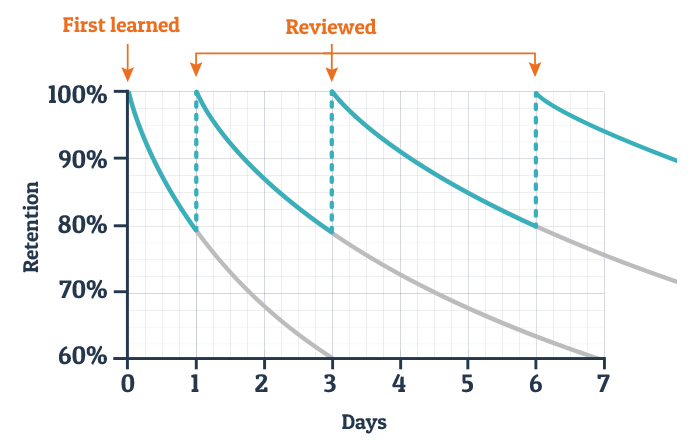
\includegraphics[width=0.5\textwidth]{figures/ebbinghaus}
\captionsetup{justification=centering}
\caption{Ebbinghaus' famous forgetting curve
\label{fig:ebbinghaus}}
\end{figure}

With this in mind I plan to iteratively build the A11Y Guide so
that the knowledge will be reinforced. The steps for its production will be
as follows:
\begin{enumerate}
  \item Search for useful resources online (First time learning)
  \item Score the identified resources with the assistive tools for a first hand
  experience along with other criteria (Second time repeating)
  \item Collate the resources under the correct header in a github project
  \item Setup continuous deployment scripts to ensure deploy on commit
  \item For each header create and document best practices (Third time
  repeating)
  \item Build a basic documentation website
  \item For each header create coded examples (Fourth time repeating)
\end{enumerate}

As explicitly stated there will be four loops of observing, reviewing and
applying the knowledge learned which should result in a peak in knowledge
when producing the tool.

\subsection{Building A11Y Guide Requirements}
In parallel to the above, for the guidance to have a greater impact it
needs to be current, relevant and available. This will require some additional
work to research the current direction the industry is moving and also the
requirements of Capgemini's teams.

\subsubsection{Understanding industry movement}
\label{sec:uim}
The purpose of understanding the current industry is to ensure that the
content within the guide is relevant and inline with the current status of the
industry. By understanding where the industry had come from and where it was
going would enable me to filter `old' resources from `new' resources and thus
produce more relevant guidance. See \ref{sec:GatheringKnowledge} for more
detail on the collection phase.

Being an apprentice within the industry I have exposure to general movements
and directions (through colleagues and self found sources), but primary
evidence was required to back up my personal opinion.

In 2016 the largest survey ever of front end developers was completed the
'State of JS' \citep{StateOfJs}. This survey covered almost every aspect of the front end
from javascript frameworks through tooling, all the way to testing frameworks.
Participants were asked to categorise technologies into the following five
pointers:
 \begin{itemize}
  \item `Used it before, would use again'
  \item `Used it before, would not use again'
  \item `Heard of it, would like to learn'
  \item `Heard of it, not interested'
  \item `Never heard of it'
 \end{itemize}

Based on my constant technology tracking I hypothesised that the technologies
that were `Used it before, would use again' and `Heard of it, would like to
learn' were the big winners in 2017. In Javscript frameworks this was ReactJs
and Angular 2. Again this needed clarification so I chose to use `Google
Trends' \citep{GoogleTrends} a tool which allows users to view graphs of
search queries on a
relative scale. During development most software engineers will
refer to google for documentation and issues so I felt this was going to be a
sound method for determining this. Fig.~\ref{fig:js_compare} confirms my
hypothesis and shows how ReactJS overtook AngularJS with Angular 2 on the rise.

\begin{figure}[H]
\centering
\centering
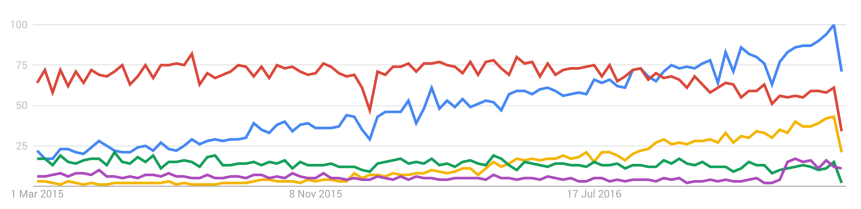
\includegraphics[width=\textwidth]{figures/js_compare}

\includegraphics[width=\textwidth]{figures/js_compare_key}
\captionsetup{justification=centering}
\caption{March 2017 Snapshot of JS Frameworks on Google Trends
\label{fig:js_compare}}
\end{figure}

\subsubsection{Questionnaire}
% TODO
% - Reference Professional competency scale https://hr.od.nih.gov/workingatnih/competencies/proficiencyscale.htm
% - Reference Remote working Capgemini
% - Reference google forms

The questionnaire's purpose is to understand the frameworks, components and
competencies in use across Capgemini. The next three paragraphs describe what
I want to discover and why.

The frameworks currently in use and those developers are competent in
\ref{q:1}, \ref{q:2}. These will be used to backup the hypothesis' made in
\label{sec:uim} and also enable me to feedback into my team on any gaps we
have within the industry.

Web Components client applications have in them \ref{q:5}. This will
determine the order in which guidance is generated in the A11Y Guide.
As I am aiming for continuous delivery, by adding the 'higher usage'
components first I will be adding value from the most valuable to the least
valuable.

The level of competency developers have in accessibility \ref{q:6}. This will
help understand the level at which to pitch the guidance (The target audience)
and will answer the question ``What level of competency can be assumed?". My
aim is to use the National Health competency scale \citep{NHComptency} to
asses this.

Google Forms was used to implement the questionnaire due to its simple
setup and integration into Google Spreadsheets which made the following
analysis much easier.

Out of a possible 69 team members 40\% (26 members) responded.

The first two questions showed how most software developers are using or are
competent in either React or AngularJS. This with the fact that
React was discovered as an upcoming technology in \ref{sec:uim} suggests the
examples in the A11Y guide should be written in React and library
recommendations made with this in mind. It is a fair assumption that
developers competent in React should be able to apply the knowledge learned
to Angular JS. Fig.~\ref{fig:current_proj} and Fig.~\ref{fig:competent_in}
are bar charts of the results given. A suprise discovery was the popularity
of JQuery as this is slowly becoming legacy.

\begin{figure}[H]
\centering
\centering
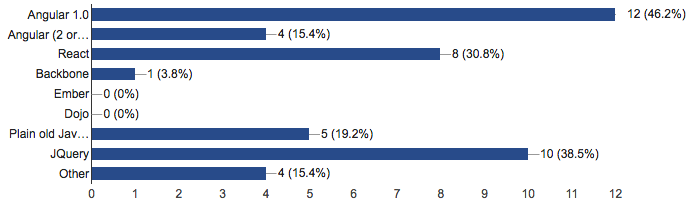
\includegraphics[width=\textwidth]{figures/questions/frameworks_in_use}
\captionsetup{justification=centering}
\caption{JS Frameworks Capgemini developers are using on current projects
\label{fig:current_proj}}
\end{figure}

\begin{figure}[H]
\centering
\centering
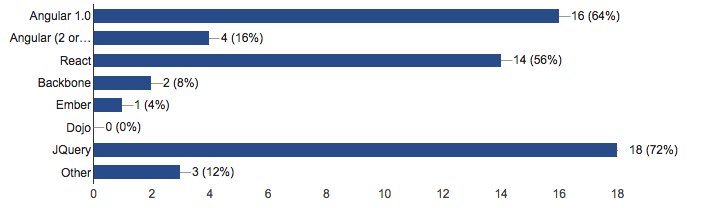
\includegraphics[width=\textwidth]{figures/questions/frameworks_competent_in}
\captionsetup{justification=centering}
\caption{JS Frameworks Capgemini developers consider themselves comfortable in
\label{fig:competent_in}}
\end{figure}

%TODO - Continue from here..



\textbf{Question 5 - What form items does your project use?}
Coming back to relevancy for the A11Y guide, content will be produced for the
highest ranking form items first. This will ensure that if the guide is not
100\% complete it will still likely add a lot of value to Capgemini.

This question will be multi-choice and list a range of different methods of
user input

\textbf{Question 6 - What Web Components does your project use?}
Similar to above accept it is probably within the scope of this project that
only the highest ranking six will have guidance produced. This may be
completed however after the project.

\textbf{Question 7 - What level would you consider your web accessibility
level?}
This question aims to have the developer place themselves on the NIH
Proficiency Scale. It will have some additional guidance to help them
position themselves:
\begin{itemize}
\item None
\item Fundamental Awareness - Know what it is, but not how to implement it
\item Novice - Can implement with help from Google
\item Intermediate - Can implement with help and has experience testing with tools such as JAWS, Dragon
\item Advanced  - Can implement without help, understands \& explains how.
Knows best practice
\item Expert - The 'go to' person for web accessibility
\end{itemize}

This is probably the most important question. The answers to this will
determine the depth to which the guidance goes into, and also it's
recommended usage.

\subsection{Gathering Knowledge}
\label{sec:GatheringKnowledge}
This section will describe the methods and results of gathering resources to
be used to support the A11Y Guide.

\subsubsection{Method}
I chose to apply a method to ensure consistency and quality. The first and
simplest method I experimented with was to collate the top five results from
'Google'. This was the obvious and quickest method to gather such information
however, after reviewing resources in 'Links' and 'Buttons' items which I am
personally familiar with. I found a lot of overlap between content and after
testing them with the tools, similar mistakes across all of them.
None seemed to capture the 'why' which naturally meant I needed a
different method.

To produce a new method I started by understanding what I needed to know to
produce the content. By understanding this I would be able to produce a method
by which I could assess an individual resources relevance and usefulness. The
key things I needed to know were:

\begin {itemize}
\item What does bad look like?
\item What do I need to do? e.g Coding Examples
\item Why should I write my code this way?
\item How do the assistive tools handle the outputs?
\item How can one test for correctness?
\end{itemize}

I produced 10 questions each with a possible score of 10. I was looking to
use the three best scoring resources in my content.

\subsubsection{Example Scoring}


\subsubsection{Outputs}
Inline with my 'Open Source' and 'Share Everything' ethos the resources were
sorted based upon their content and placed upon my github account in a public
 repository.
See Fig \ref{fig:allyLinksDemo}.
Following the principles of Continuous Delivery this could in fact be
considered the v1.0.0 of my A11Y Guide.

\begin{figure}[H]
\centering
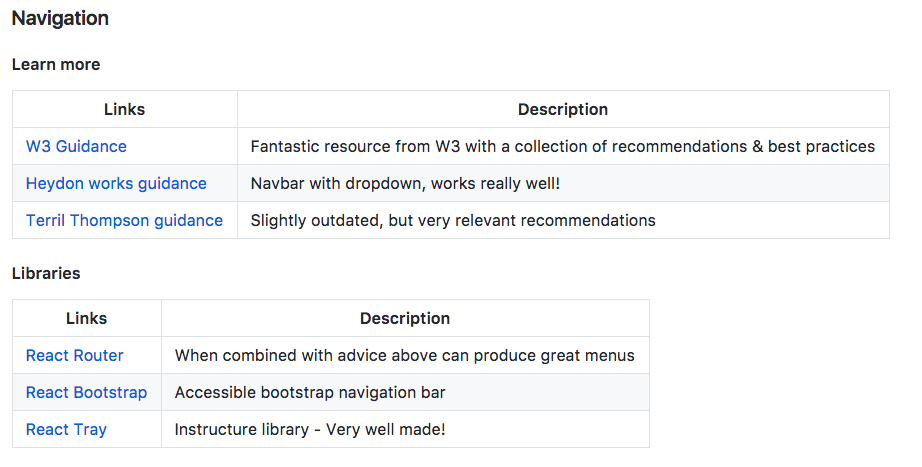
\includegraphics[width=\textwidth]{figures/documentation_link_example}
\captionsetup{justification=centering}
\caption{A demonstration of the 'Navigation' content on Github.
https://github.com/Geeman201/a11y-links/
\label{fig:allyLinksDemo}}
\end{figure}


\subsubsection{Defining Requirements}
% TODO - Reference Dan North https://dannorth.net/whats-in-a-story/
From the questionnaire, common web frameworks, knowledge gained from the
resources and inline with my manifesto I started to write down concrete
requirements. I used Dan North's "What's in a Story" method to write the
requirements. I find this method gives both 'the what' and 'the why' which
enables a better decision making process to be followed. As an additional
benefit in this format I have a solid means by which I can evaluate the
solution later.

\begin{center}
 \begin{tabular}{| c |}
 \hline
 As a developer \\
 \hline
 I want to have a section highlighting the most important aspects I need to
 understand \\
 So that when I come to refresh my skills I only have to read that section  \\
 \hline
 I want to have coded examples written in React \\
 So that I can understand and apply the knowledge \\
 \hline
 I want to have audio/subtitled examples of how the tools behave  \\
 So that I know the impact (The why) of Good/Bad semantics  \\
 \hline
 I want relevant links available  \\
 So that I can find more information out  \\
 \hline
\end{tabular}
\end{center}

\section{Deliverable}
% TODO -
% Reference Markdown -
% Reference Github - https://github.com/open-source
\subsection{Iteration 1 - Create content using markdown}
The first iteration of developing content was targetted the broader aspects
which affect every part of the experience. This covered page structure,
page content and other general aspects like typography and colour. The content was produced
using markdown.

\subsubsection{Why Markdown?}
Markdown was chosen as it is fast becoming the 'developer standard' for writing
documentation. When producing content, familiarity is key to producing an
enviornment in which people will collaborate. If you first have to
learn a new language or tool the barrier to entry to produce the content is
higher and thus you are less likely to do it. As Github the 'worlds biggest'
software control platform has bought into markdown as way developers communicate
'most' developers have at least some knowledge in the area. If they do not,
the documentation for using markdown is well estabilished.

An additional benefit to using markdown is it is relatively difficult to make
the content you produce "Inaccessible". As I want the guide to demonstrate
best practices; it should really be following them. Markdown compilers are
great at transforming content into 'assistive tool' friendly HTML.

Fig \ref{fig:hierarchy} and Fig \ref{fig:structures} demonstrates how the
content is displayed in github's standard folder view. The markdown text is
converted into HTML and displayed in a clear well structured manner.

\begin{figure}[H]
    \centering
    \begin{subfigure}[b]{0.25\textwidth}
        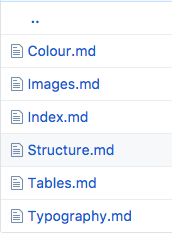
\includegraphics[width=\textwidth]{figures/documentation_md_example_1}
        \captionsetup{justification=centering}
        \caption{The File Hierarchy of 'Content' section}
        \label{fig:hierarchy}
    \end{subfigure}
    \qquad
    %add desired spacing between images, e. g. ~, \quad, \qquad, \hfill
      %(or a blank line to force the subfigure onto a new line)
    \begin{subfigure}[b]{0.4\textwidth}
        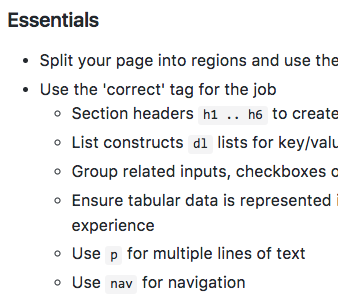
\includegraphics[width=\textwidth]{figures/documentation_md_example_2}
        \captionsetup{justification=centering}
        \caption{The 'structures.md' file rendered in the browser}
        \label{fig:structures}
    \end{subfigure}
\end{figure}

\subsection{Iteration 2 - UI Design \& Build site}
I wanted the UI to be simple and follow all the best practices it recommends.
As I had written some content it made it easier to experiment and understand
what was needed. The content was structured almost as a hierarchichal tree so
some sort of accordian type navigation would be useful. The audio snippets
would need to supplement the main content. The code snippets
would need to be embeddedable in the page.

I used moqups to produce a three different designs.
% TODO
% - Reference mockups
Design 1:

Design 2:

Design 3:

I chose design...

From the user interface design I produced a system design See Fig
\ref{fig:allycomponent}. As the content was held in markdown files the
dcumentation framework would only have to parse the markdown and generate a
navbar and HTML. The idea was to enable the documentation framework
to be reused by abstracting the framework away from the content itself. For a
user of the documentation framework, I wanted them to only have to edit the
content and/or the Table of Contents. This would enable content to be the
users main focus and thus speed up the development of the guide.
\begin{figure}[H]
\centering
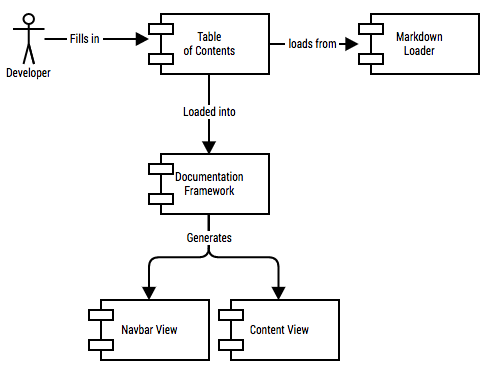
\includegraphics[width=0.65\textwidth]{figures/documentation_design}
\captionsetup{justification=centering}
\caption[Short figure name.]{Component Diagram for A11Y Guide
\label{fig:allycomponent}}
\end{figure}
A table of contents was
chosen rather than browsing folder structures so that users
could be in control of the ordering on the navbar. The table of contents
would be a JSON array with each object containing the following data:
\begin{itemize}
\item label - This would be the title of the page
\item url - This would be the path so content could be linked to directly
\item component - The markdown file to render
\item children - An array of children pages with the same JSON object structure.
\end{itemize}
A side effect of this design which was only realised in Iteration 4 was the
added benefit of extensibility and customisability of labels, url paths and
components. See \ref{sec:iteration_4} for how this design enabled custom
components to be used.

\subsection{Iteration 3 - Continue content}
As described by the title this iteration focussed on producing more content;
specifically around forms and components.

\subsection{Iteration 4 - Recognise/Implement custom pages}
\label{sec:iteration_4}
The more content that was written the greater the need for the ability to
insert custom content. I was finding myself working around the drawbacks of
markdown when creating examples with custom HTML, JS and CSS. This became a
real problem when filling out content for the components section. I decided
to alter the code to enable React Components to be injected. How these
slotted into the design is
shown in \ref{fig:allycomponent_2}. Note how the rest of the documentation
framework didn't have to change!

\begin{figure}[H]
\centering
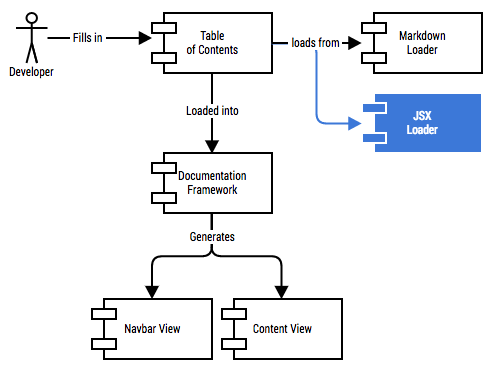
\includegraphics[width=0.65\textwidth]{figures/documentation_design_2}
\captionsetup{justification=centering}
\caption[Short figure name.]{Component Diagram for A11Y Guide with added JSX
component loader highlighted in blue.
\label{fig:allycomponent_2}}
\end{figure}

\subsection{Iteration 5 - Continue content}
This iteration involved adding coded examples to areas where markdown was not
appropriate.

\subsection{Iteration 6 - Generify}
This iteration focussed on extracting the common documentation framework that
had been produced. Removing the content and setting up a different repository
which others could clone and create their own documentation from.

\section{Extending the impact}
\subsection{Markdown/React Documentation Framework}
\subsection{Colour Contrast Tool}
% TODO
%  * Refernce CSS in JS
%  * Reference Anti CSS in JS movemtn
%  * Reference Max
Whilst I was creating the A11Y Guide I was asked to experiment with an
upcoming piece of technology. "CSS in JS". The industry has been moving
towards 'component driven' development through the entrance of Angular and
ReactJS; CSS in JS is the last step in all code relating to a
component being co-located in a single file. Myself like others had had
significant reservations about the performance and portability of such an
idea. However, working for a technology consultancy firm we are advised to
form an opinion on any impacting changes within our retrospective spaces.

% TODO - Reference Juicy Studio/Snook
Having done research into colour contrast tools I identified a gap for a
"modern", user focussed tool. Most current tools require submission to a
server and lack demonstrations of what the two colours look like when used
together. All of them satisfied a relatievly simple set of requirements:
\begin{itemize}
\item Report the colour contrast level between two distinct colours
\item Report whether the colours contrast level of such colours satisfies the
 WCAG guidelines for the "wanted" text size.
\end{itemize}

%TODO - Reference Moqups
Using Moqups again I quickly put together a quick design using their colour
schemes and fonts See \ref{fig:colour_contrast_1}. To test out "CSS in JS" I
wanted to use 'Styled Components' a ReactJS implementation written by Max
Stoblier. ``Create React App" a tool for bootstrapping a React project was also
used. This was only an `experiment' and thus to be completed quickly, testing
was reduced to cover only the core logic for calculating colour contrast.

\begin{figure}[H]
\centering
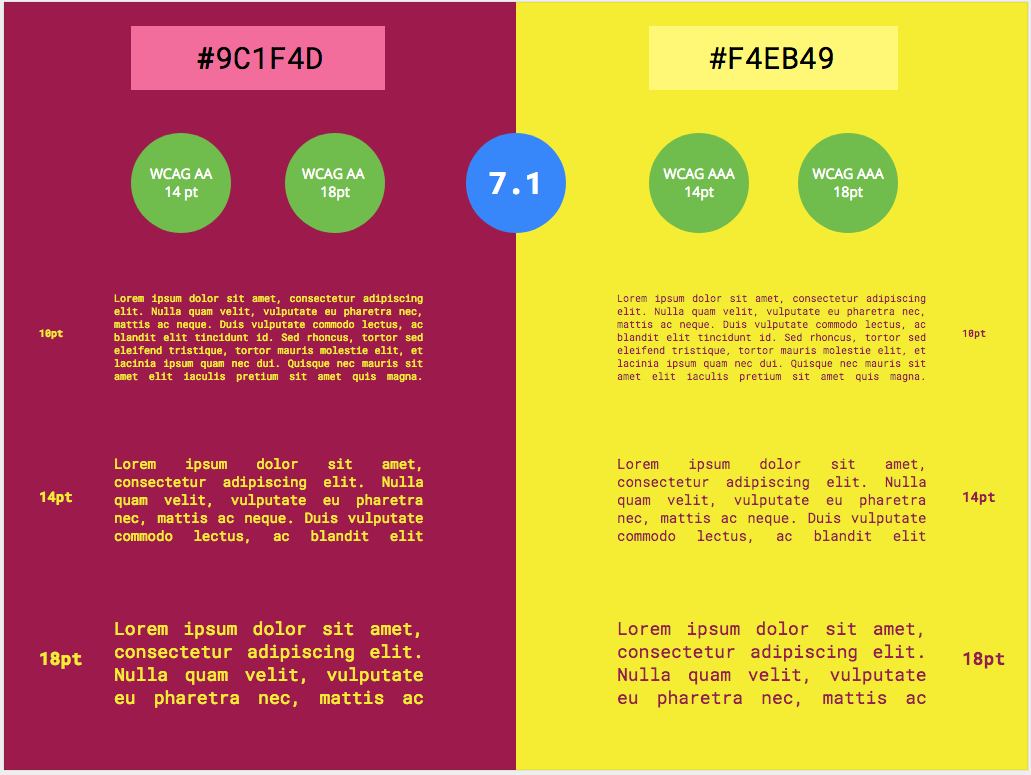
\includegraphics[width=0.65\textwidth]{figures/colour_contrast_1}
\captionsetup{justification=centering}
\caption{Design for Colour Contrast tool
\label{fig:colour_contrast_1}}
\end{figure}

The 'Happy Day' user journey would be:
\begin{itemize}
\item User enters first colour in input field (Can paste)
\item User enters second colour in input field
\item On a valid colour entered. Both are displayed as background and
foreground; the value of colour contrast is displayed; and the contrast
levels WCAG appropriateness is displayed in the circles. Green for success, Red
for failure.
\end{itemize}

In the error scenario of a user entering an invalid colour, the background
colours would remain the same and the input field would have a 'red'
background and border to signify an error.

% TODO - discuss Travis CI for report writing
% TODO - discuss Branching model
% TODO - discuss any Standards


Principally, this chapter should describe the work that was undertaken before
code was written, hardware built, theories worked on, or research studies
executed. It should show how the project proposal was further refined and
clarified, so that the implementation/research execution stage could go
smoothly rather than by trial and error. This part of the report is attempting to
prove that you went through a planning process before embarking on the
deliverable so among others it might include discussion of:

1. For software projects, a requirements analysis, HCI designs, architectural
and use-case diagrams, etc.
2. Any programming languages learnt, any complicated theories or algorithms
that required understanding
3. For research-based projects, the research approach (experimental design,
where applicable), including methods and tools that were used/applied. If the
research method involves the development of prototypic software to test a
concept, briefly describe the design, structure, and creation of this software.
Research methods should be described such that a third party could replicate
the study/experiment to validate the results.

This section should be answering the question “How did I plan to achieve the
deliverable?”
